\section{Organisation du projet}
\subsection{Structure d’organisation}
L'équipe est composée de quatre membres.
% TODO lister fonction des membres
\begin{itemize}
	\item Badre Baba ;
	\item Geoffroy Carrier ;
	\item Jean-Christophe Saad-Dupuy ;
	\item Scheer Mickael.
\end{itemize}

%\subsection{Interfaces externes}
\subsection{Rôles et Responsabilités}
\begin{figure}[thbp]
	\centering
		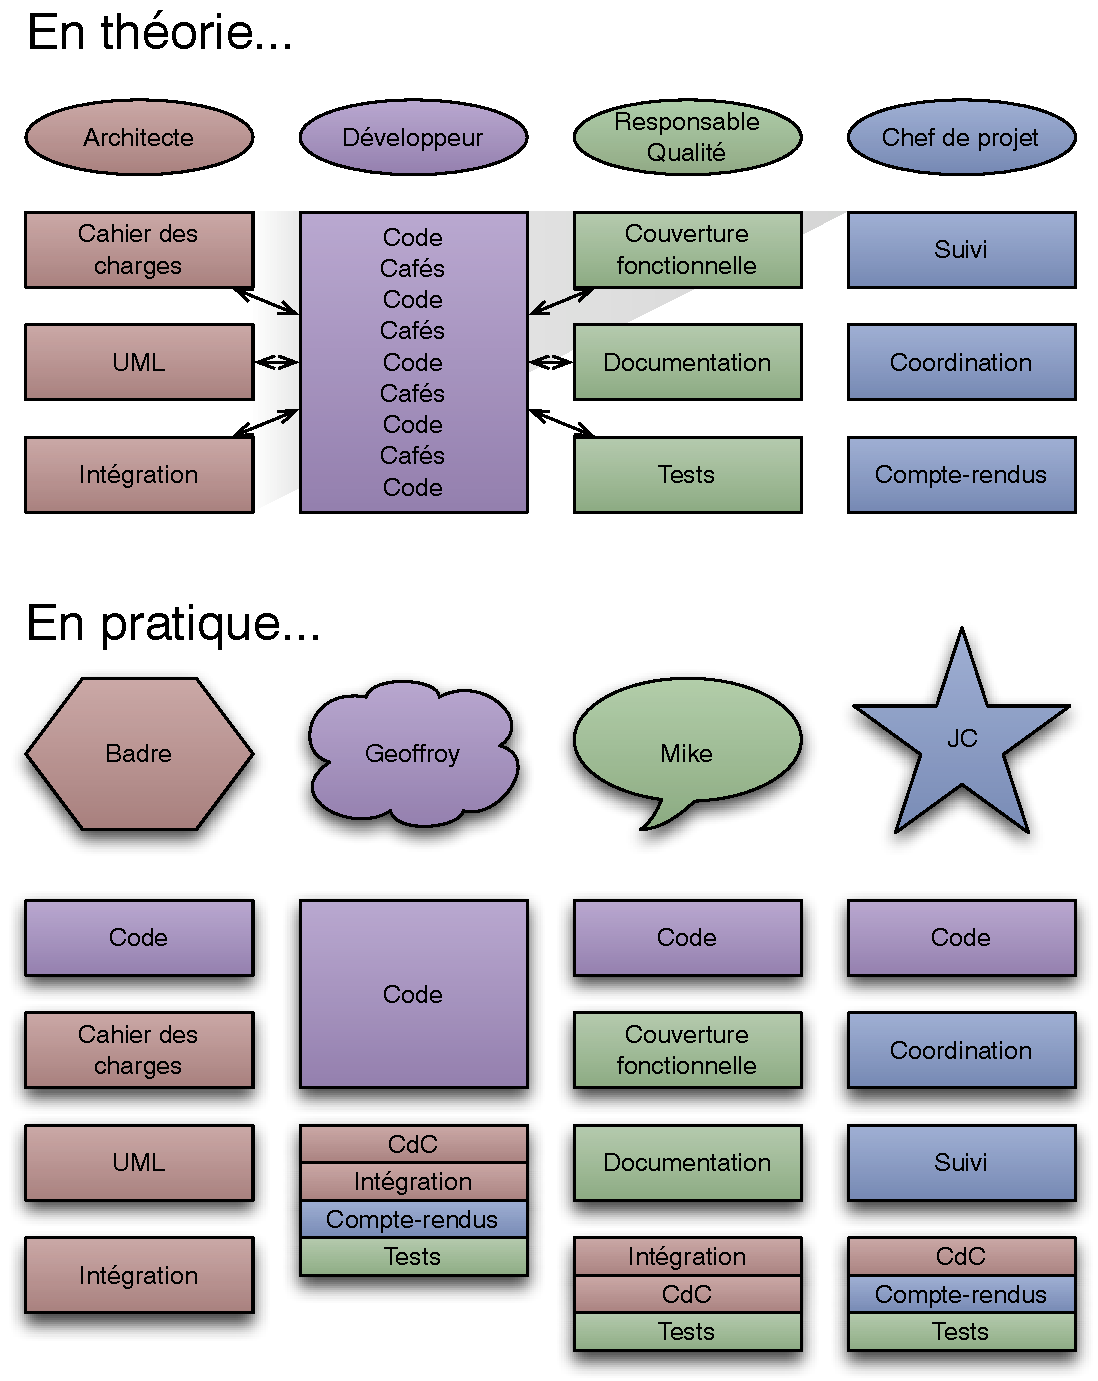
\includegraphics[width=15cm]{../diagrammes/repartition_taches.pdf}
	\caption{Répartition des tâches}
	\label{fig:repartition}
\end{figure}

Nous avons répartis les tâches de chaque intervenant de notre équipe en adaptant les différentes responsabilité des postes attribués, tout en respectant les aspirations de chaque membre de l'équipe comme en témoigne la figure~\ref{fig:repartition}.
